\documentclass[tikz,border=2pt]{standalone}
\usepackage{amsmath,amssymb}
\usepackage{tikz}
\usetikzlibrary{arrows.meta}

\begin{document}
% Row operations replace a system by an equivalent one: different lines, same solution set.
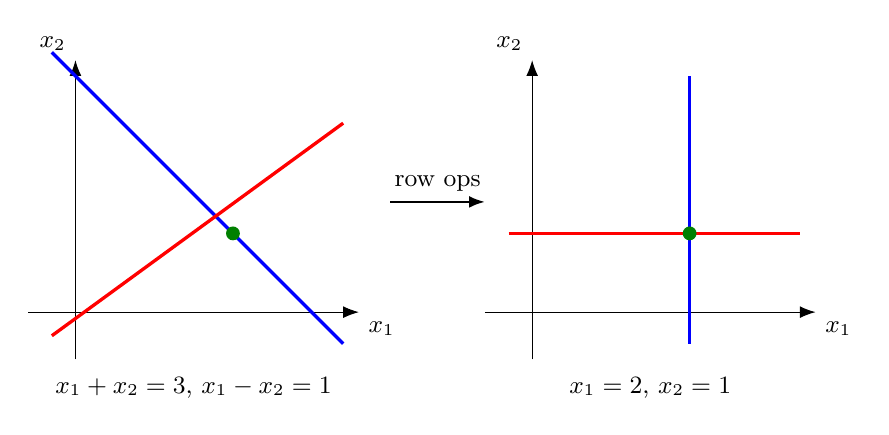
\begin{tikzpicture}[every node/.style={font=\small}, >={Latex[length=2mm]}]
	\begin{scope}
		\draw[->] (-0.6,0) -- (3.6,0) node[below right] {$x_1$};
		\draw[->] (0,-0.6) -- (0,3.2) node[above left] {$x_2$};
		\draw[blue, very thick] (-0.3,3.3) -- (3.4,-0.4);
		\draw[red, very thick] (-0.3,-0.3) -- (3.4,2.4);
		\fill[green!50!black] (2,1) circle (2.5pt);
		\node[anchor=north, align=center] at (1.5,-0.7) {$x_1+x_2=3$,\ $x_1-x_2=1$};
	\end{scope}
	\draw[->, thick] (4.0,1.4) -- (5.2,1.4) node[midway, above, font=\small] {row ops};
	\begin{scope}[xshift=5.8cm]
		\draw[->] (-0.6,0) -- (3.6,0) node[below right] {$x_1$};
		\draw[->] (0,-0.6) -- (0,3.2) node[above left] {$x_2$};
		\draw[blue, very thick] (2,-0.4) -- (2,3.0);
		\draw[red, very thick] (-0.3,1) -- (3.4,1);
		\fill[green!50!black] (2,1) circle (2.5pt);
		\node[anchor=north, align=center] at (1.5,-0.7) {$x_1=2$,\ $x_2=1$};
	\end{scope}
\end{tikzpicture}
\end{document}
